\documentclass[letterpaper,headings=standardclasses]{scrartcl}

\usepackage[margin=1in,includefoot]{geometry}
\usepackage{amssymb}
\usepackage{amsmath}
\usepackage{listings}
\usepackage{tikz}
\usepackage{float}

\usetikzlibrary{shapes,arrows}

\tikzset{
  block/.style    = {draw, thick, rectangle, minimum height = 3em, minimum width = 3em},
  sum/.style      = {draw, circle},
  input/.style    = {coordinate, circle},
  output/.style   = {coordinate, circle},
  neuron/.style   = {draw, thick, circle, minimum height = 3em, minimum width = 3em}
}

\lstset{basicstyle=\ttfamily,language=python,columns=flexible,breaklines=true}

\title{Homework 2}
\subtitle{CS 559 - Neural Networks - Fall 2019}
\author{Matteo Corain 650088272}

\begin{document}

\maketitle

\section{Question 1}

\subsection{General architecture of the network}

In order to design a network capable of implementing the proposed separation, it is possible to proceed as follows:

\begin{itemize}

\item First, we need to identify the inequalities that describe the two regions and implement them using a set of perceptrons;

\item Then, since the inequalities for the two regions should be all satisfied at once, we need to connect the outputs of all perceptrons useful for describing a region using a perceptron implementing a logical AND;

\item Finally, since the output of the network should be positive in case the pattern belongs to any of the two regions, we need to connect the outputs of the AND perceptrons using a perceptron implementing a logical OR.

\end{itemize}

Let us first begin to identify the linear relationships that are necessary to identify the colored regions. Using the nomenclature shown in figure \ref{region_names}, we have:

\begin{figure}[h]
\centering
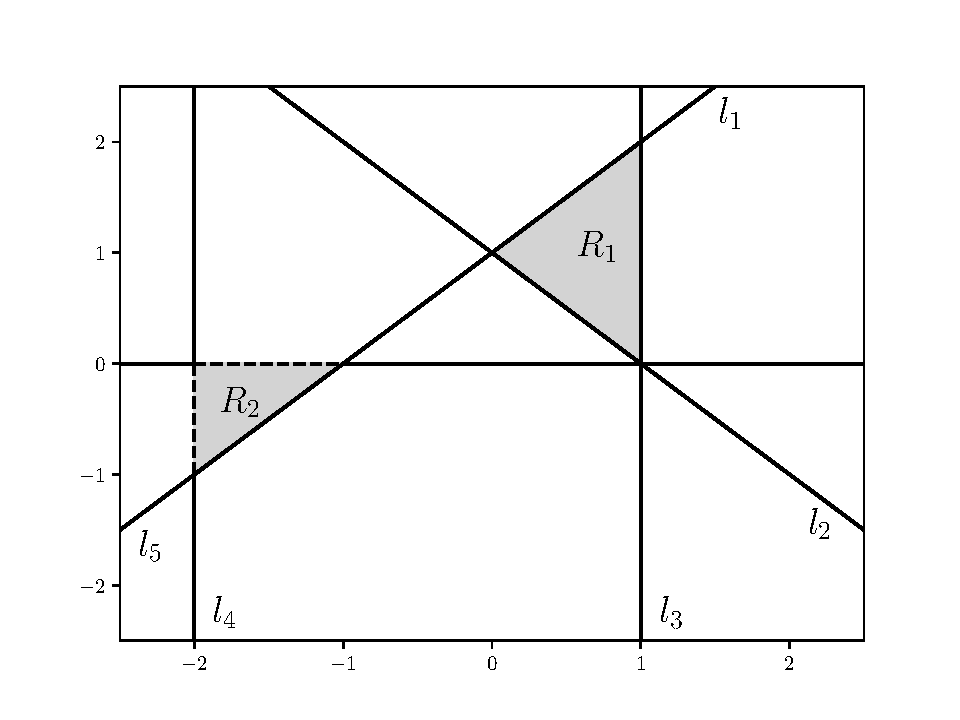
\includegraphics[width=.7\linewidth]{region_names.pdf}
\caption{Nomenclature used for lines and regions}
\label{region_names}
\end{figure}

$$ l_1 : - 1 - x + y = 0, \quad l_2 : -1 + x + y = 0 $$
$$ l_3 : -1 + x = 0, \quad l_4: 2 + x = 0, \quad l_5 : y = 0 $$

Given this nomenclature, the two regions are described by the following set of inequalities:

$$ R_1 = \begin{cases} l_1 \le 0 \\ l_2 \ge 0 \\ l_3 \le 0 \end{cases}, \quad R_2 = \begin{cases} l_1 \ge 0 \\ l_4 > 0 \\ l_5 < 0 \end{cases} $$

As it can be seen, some of these inequalities do not present the equality sign; since the perceptrons we are designing use the step activation function (which returns 1 when the pattern is on the separator), this means that those cannot be implemented by a single perceptron. Instead, we have to make use of a succession of two perceptrons, the first implementing the complimentary inequality and the second implementing a logical NOT:

$$ l_4 > 0 \Rightarrow \neg (l_4 \le 0), \quad l_5 < 0 \Rightarrow \neg (l_5 \ge 0) $$

The block diagram of the network to implement is shown in figure \ref{blk_diagram}; each block represents a perceptron to be designed. As we can see, the network is composed of four distinct layers:

\begin{itemize}

\item The first layer is the \emph{line layer}, and includes the neurons used to implement the separation described by the linear inequalities;

\item The second layer is the \emph{NOT layer}, and includes the neurons used to implement the NOT operation as requested by inequalities not including the equality sign; for inputs that do not need the usage of a NOT perceptron, we can imagine that those are connected to a buffer perceptron, simply returning as output the input value;

\item The third layer is the \emph{AND layer}, and includes the neurons used to implement the AND operation among inequalities useful to describe the same region (all should be satisfied at the same time);

\item The fourth layer is the \emph{OR layer}, and includes the neuron used to implement the OR operation among the results of the previous layer (we want a positive result if the pattern is either in $R_1$ or in $R_2$).

\end{itemize}

\begin{figure}[H]
\centering
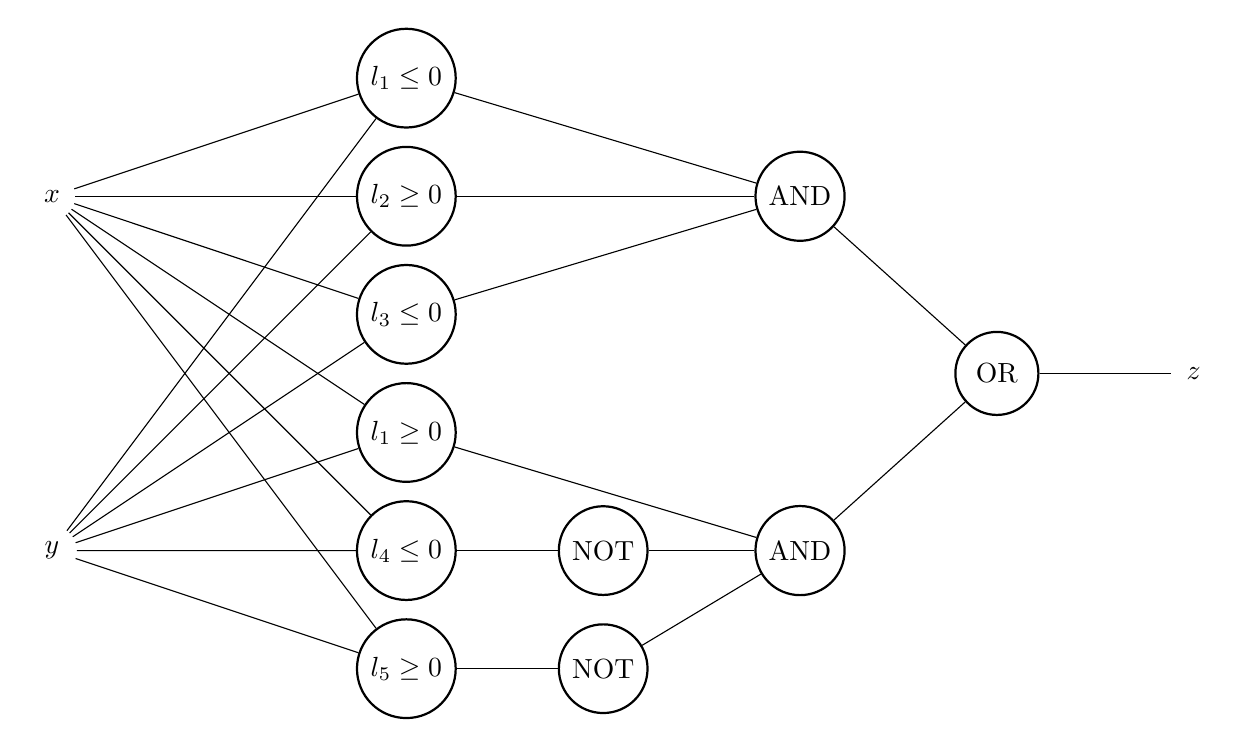
\begin{tikzpicture}[auto, node distance=1.5cm, >=triangle 45]

% Input layer
\draw node [input, name=x] {$x$};
\draw node [input, name=y, below of=x, node distance=4.5cm] {$y$};

% First layer
\draw node [neuron, right of=x, yshift=1.5cm, node distance=4.5cm] (p11) {$l_1 \le 0$};
\draw node [neuron, below of=p11] (p12) {$l_2 \ge 0$};
\draw node [neuron, below of=p12] (p13) {$l_3 \le 0$};
\draw node [neuron, below of=p13] (p14) {$l_1 \ge 0$};
\draw node [neuron, below of=p14] (p15) {$l_4 \le 0$};
\draw node [neuron, below of=p15] (p16) {$l_5 \ge 0$};

% Second layer
\draw node [neuron, right of=p15, node distance=2.5cm] (p21) {NOT};
\draw node [neuron, right of=p16, node distance=2.5cm] (p22) {NOT};

% Third layer
\draw node [neuron, right of=p12, node distance=5cm] (p31) {AND};
\draw node [neuron, right of=p21, node distance=2.5cm] (p32) {AND};

% Fourth layer
\draw node [neuron, right of=p31, yshift=-2.25cm, node distance=2.5cm] (p41) {OR};

% Output
\draw node [output, name=z, right of=p41, node distance=2.5cm] {$z$};

% Connections
\draw[-](x) -- node {}(p11);
\draw[-](x) -- node {}(p12);
\draw[-](x) -- node {}(p13);
\draw[-](x) -- node {}(p14);
\draw[-](x) -- node {}(p15);
\draw[-](x) -- node {}(p16);
\draw[-](y) -- node {}(p11);
\draw[-](y) -- node {}(p12);
\draw[-](y) -- node {}(p13);
\draw[-](y) -- node {}(p14);
\draw[-](y) -- node {}(p15);
\draw[-](y) -- node {}(p16);

\draw[-](p15) -- node {}(p21);
\draw[-](p16) -- node {}(p22);

\draw[-](p11) -- node {}(p31);
\draw[-](p12) -- node {}(p31);
\draw[-](p13) -- node {}(p31);
\draw[-](p14) -- node {}(p32);
\draw[-](p21) -- node {}(p32);
\draw[-](p22) -- node {}(p32);

\draw[-](p31) -- node {}(p41);
\draw[-](p32) -- node {}(p41);

\draw[-](p41) -- node {}(z);

\end{tikzpicture}
\caption{Block diagram of the requested network}
\label{blk_diagram}
\end{figure}

\subsection{Line neurons}

Line neurons constitute the first layer of the network; they receive two inputs, namely the $x$ and $y$ inputs of the network, and return a binary output that is positive when the pattern satisfies the associated inequality. In order to design them correctly, we have to recall what kind of class separation a perceptron with step activation in general implements; for the case with two inputs $x$ and $y$, this is expressed in the normal form:

$$ w_0 + w_1x + w_2y \ge 0 $$

Therefore, if we can write the inequalities that describe the regions for which we want a positive output in a form that matches the normal one, it is possible to derive the vector of weights $w$ of the perceptron directly from the inequality itself. Using this procedure, the following results can be obtained:

\begin{itemize}

\item Neuron \#1: for the first neuron, the inequality to implement is $-1 -x +y \le 0$, which is, in normal form, $1 +x -y \ge 0$; thus, a possible choice of weights for this neuron is:

$$ w_1 = [\begin{matrix} 1 & 1 & -1 \end{matrix}] $$

\item Neuron \#2: for the second neuron, the inequality to implement is $-1 +x +y \ge 0$, already in normal form; thus, a possible choice of weights for this neuron is:

$$ w_2 = [\begin{matrix} -1 & 1 & 1 \end{matrix}] $$

\item Neuron \#3: for the third neuron, the inequality to implement is $-1 +x \le 0$, which is, in normal form, $1 -x \ge 0$; thus, a possible choice of weights for this neuron is:

$$ w_3 = [\begin{matrix} 1 & -1 & 0 \end{matrix}] $$

\item Neuron \#4: for the fourth neuron, the inequality to implement is $-1 -x -y \ge 0$, already in normal form; thus, a possible choice of weights for this neuron is:

$$ w_4 = [\begin{matrix} -1 & -1 & 1 \end{matrix}] $$

\item Neuron \#5: for the fifth neuron, the inequality to implement is $2 +x \le 0$, which is, in normal form, $-2 -x \ge 0$; thus, a possible choice of weights for this neuron is:

$$ w_5 = [\begin{matrix} -2 & -1 & 0 \end{matrix}] $$

\item Neuron \#6: for the sixth neuron, the inequality to implement is $y \ge 0$, already in normal form; thus, a possible choice of weights for this neuron is:

$$ w_6 = [\begin{matrix} 0 & 0 & 1 \end{matrix}] $$

\end{itemize}

\subsection{NOT neurons}

NOT neurons constitute the second layer of the network; they receive a single input, namely the output of a line neuron, and return the logical inverse of that input. If we suppose that the network topology has to be complete, i.e. each neuron is connected to the output of each neuron in the previous layer, then it is possible to suppose that the weights relative to the unused inputs are set to 0. They can be implemented using the standard set of weights:

$$ w = [\begin{matrix} 0.5 & -1 \end{matrix}] $$

Not all line perceptrons need to be negated for implementing the requested network. If we want to build a complete layer of neurons, we can imagine to introduce a set of “buffer” neurons, which simply return as output the received input; these can be implemented using the following set of weights that is opposite to the one of the NOT neurons:

$$ w = [\begin{matrix} -0.5 & 1 \end{matrix}] $$

\subsection{AND neurons}

The two AND neurons constitute the third layer of the network; they both receive three inputs, namely the outputs of the line neurons (possibly negated) that describe a single region, and return a binary output that is positive when the pattern is located inside the region (all inequalities are satisfied at once). They can be implemented using the standard design procedure:

\begin{itemize}

\item The bias $w_0$ is set to $-n_i+0.5$, where $n_i$ is the number of inputs of the perceptron;

\item Weights $w_1,\dots,w_{n_i}$ are set to 1.

\end{itemize}

In this case, therefore, both AND neurons may use the following set of weights:

$$ w = [\begin{matrix} -2.5 & 1 & 1 & 1 \end{matrix}] $$

Also in this case, if we assume that the network topology has to be complete, weights corresponding to unused inputs may be set to 0.

\subsection{OR neuron}

The single OR neuron constitute the fourth and last layer of the network; it receives two inputs, namely the outputs of the two AND neurons, and returns a binary output that is positive when the pattern is located inside one of the two regions. It can be implemented using the standard design procedure:

\begin{itemize}

\item The bias $w_0$ is set to $-0.5$;

\item Weights $w_1,\dots,w_{n_i}$ are set to 1.

\end{itemize}

In this case, therefore, the OR neuron may use the following set of weights:

$$ w = [\begin{matrix} -0.5 & 1 & 1 \end{matrix}] $$

\subsection{Network testing}

\begin{figure}[H]
\centering
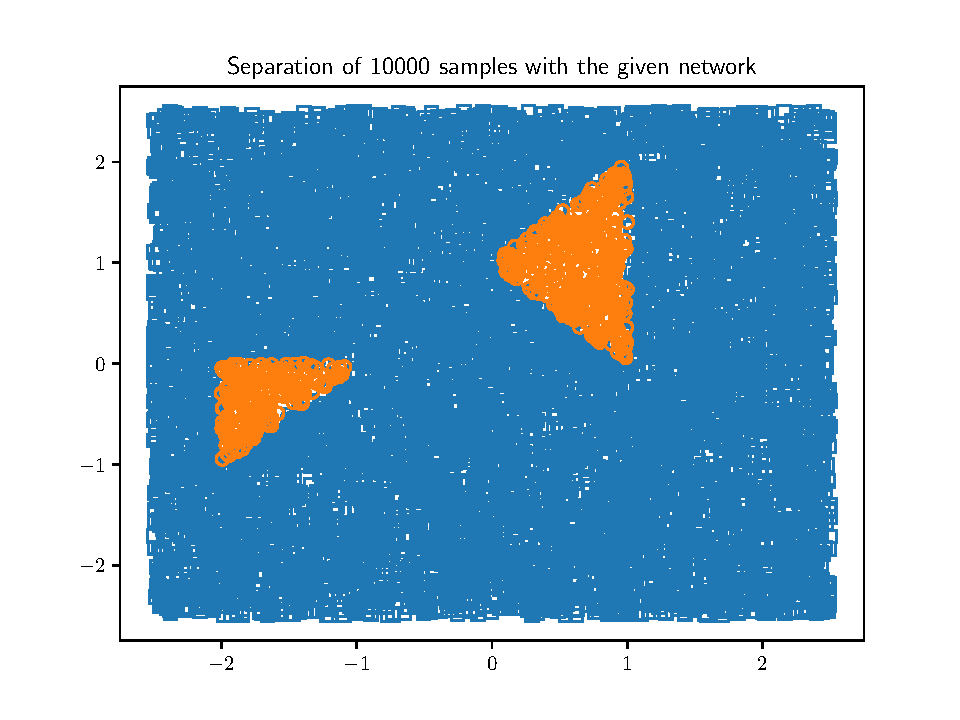
\includegraphics[width=.7\linewidth]{sep_10000.pdf}
\caption{Separation of 10000 samples with the given network}
\label{sep_10000}
\end{figure}

% The described network has been implemented in a computer program and used to classify 10000 random samples $x_i \in [-2.5, 2.5]^2$. Results are shown in figure \ref{sep_10000}.

\section{Question 2}

\subsection{Parsing of the input files}

The first step to take for the sake of the exercise is to parse the input files, encoded using the binary IDX format, into Numpy arrays that can be used to train the network using the multicategory PTA. As described in the provided website, those files are structured according to the following scheme:

\begin{itemize}

\item The first four bytes represent the \emph{magic number}, which has the following meaning:

\begin{itemize}

\item The first two bytes are identically set to 0;

\item The third byte identifies the type of the data stored in the file, which is in this case \emph{unsigned integer} (associated to the hexadecimal value 0x08);

\item The fourth byte identifies the \emph{number of dimensions} of the stored data, which is set to 1 for the labels files (single vector containing all the labels) and to 3 for the images files (vector containing a list of 2-dimensional matrices).

\end{itemize}

In this case, the magic number is therefore set to decimal value 2051 for images files and to decimal value 2049 for labels files.

\item The following four bytes tell how many items are present in the collection; this is set to 60000 for training files and to 10000 for test files;

\item In the images files, the following pair of 4-bytes integers explicit the width and height of the samples (in this case, they are 28 pixels by 28 pixels);

\item The following bytes represent the data to be parsed.

\end{itemize}

All numeric values are stored using the \emph{big endian} format, which means that the most significant bytes are stored at lower offset values. In order to parse the images and labels files, two separate functions have been coded:

\begin{itemize}

\item Function \texttt{idx\_images\_parse()} is used to parse the images files encoded in the IDX format; it performs the following actions:

\begin{itemize}

\item It opens the given file in \emph{read binary} mode;

\item It reads the magic number using the \texttt{fromfile()} function provided by the Numpy library, which allows to read a certain number of elements (in this case, a single one) from a file given their data type (in this case, big endian \texttt{>}, unsigned integer \texttt{u} on four bytes \texttt{4}) and checks its correctness (it must be equal to 2051);

\item In the same way, it reads the number of items and the dimensions of the input images into variables \texttt{n\_samples}, \texttt{n\_rows} and \texttt{n\_cols};

\item Using the list comprehension syntax provided by the Python language and the \texttt{fromfile()} function provided by the Numpy library, it reads \texttt{n\_samples} arrays of \texttt{n\_rows * n\_cols} elements stored as big endian, unsigned 8-bits integers (\texttt{>u1}), reshapes them to the correct format and stores them into the \texttt{samples} variable;

\item It returns variables \texttt{n\_samples}, \texttt{n\_rows}, \texttt{n\_cols} and \texttt{samples}.

\end{itemize}

\item Function \texttt{idx\_labels\_parse()} is used to parse the labels files encoded in the IDX format; it performs similar actions with respect to the previous one, the only differences being that in this case samples dimensions are not present and that data items are represented by single 8-bits elements.

\end{itemize}

\subsection{Running the multicategory PTA algorithm}

The multicategory Perceptron Training Algorithm has been coded as a separate function, called \texttt{multcat\_pta()}. It takes as arguments the list of training samples (\texttt{train\_samples}), the list of training labels (\texttt{train\_labels}), the initial weights matrix (\texttt{start\_weights}), the number of samples to use (\texttt{n}), the value of $\eta$ (\texttt{eta}), the value of $\epsilon$ (\texttt{eps}) and the maximum number of epochs for which the algorithm can run (\texttt{max\_epochs}); it returns the computed weights, the number of epochs needed and the number of classification errors per epoch. This function performs the following actions:

\begin{itemize}

\item It creates a copy of the initial weights into the \texttt{weights} matrix and initializes the \texttt{epochs} variable to 0;

\item It allocates the \texttt{errors} list, which is initialized with the number of classification errors obtained using the initial weights; those are computed by using the \texttt{count\_errors()} function, which performs the sum of the elements of a list (created using the list comprehension syntax) that are set to 1 when the computed label is different from the expected label (extracted from the vector $v = Wx_i$ by means of the \texttt{array\_to\_label()} function, which simply returns the index of the component with the maximum value by means of the \texttt{argmax()} function of the Numpy library);

\item It loops until either the proportion of misclassified samples falls below the given value of $\epsilon$ or the maximum number of epochs has been reached; at each iteration, the following actions are taken: 

\begin{itemize}

\item The number of epochs is incremented;

\item The weights matrix is updated once for each training sample, by adding to it the quantity $\eta (d(x_i) - u(Wx_i)) x_i^T$; vector $d(x_i)$ is created using \texttt{label\_to\_array()}, which creates a binary array having as its only component set to 1 the one with the index given by the label, while function $u(\cdot)$ has been implemented using the \texttt{heaviside()} function of the Numpy library;

\item The number of classification errors obtained using the updated weights, computed using the already described \texttt{count\_errors()} function, is appended to the \texttt{errors} list.

\end{itemize}

\item When the loop terminates, the values of \texttt{weights}, \texttt{epochs} and \texttt{errors} are returned.

\end{itemize}

The number of classification errors per epoch may then be plotted using the \texttt{plot\_errors()} function, which creates a Matplotlib figure, plots the data, sets the title of the graph, enables the grid and shows the graph without blocking the execution.

\subsection{Results for variable $n$}

For the first part of the exercise, the multicategory PTA has been used to train a network having fixed the values of $\eta = 1$, of $\epsilon = 0$ and of an initial weight matrix $W_0$ to a set of random values in $[-1, 1]$. The only variable in the three cases has been the number of training samples $n$ that the algorithm had to use, which was set to 50, 1000 and 60000 (the entire set) in the three runs. Results are shown in table \ref{results_varn}.

\begin{table}[h]
\centering
\begin{tabular}{|c|c|c|}
\hline
$n$   & Epochs for convergence & Test set errors \\ \hline
50    & 4  & 4361 (43.610\%) \\ \hline
1000  & 43 & 1738 (17.380\%) \\ \hline
60000 & -  & 1554 (15.540\%) \\ \hline
\end{tabular}
\caption{Results for the runs with variable $n$}
\label{results_varn}
\end{table}

The algorithm was able to reach convergence both for $n = 50$ and for $n = 1000$ in a relatively low number of epochs (4 and 43, respectively); this means that the trained network is able to classify correctly all the considered items of the training set (since $\epsilon$ is set to 0). However, the performances of the network are very poor, especially for $n = 50$: when the obtained set of weights is used to classify the patterns in the test set, in fact, we get a significant proportion of misclassified items.

This may be justified by the small dimensions of the data sets used for training: the separation obtained via this kind of network, in fact, may be sufficient for the classification of a reduced training set, but it may be quite different from the “optimal” one. In other words, the computed sets of weights are able to correctly discriminate the few data points in the training set (that means that the algorithm worked correctly), but they are unable to correctly classify large numbers of objects (the separation is not optimal).

\begin{figure}[h]
\centering
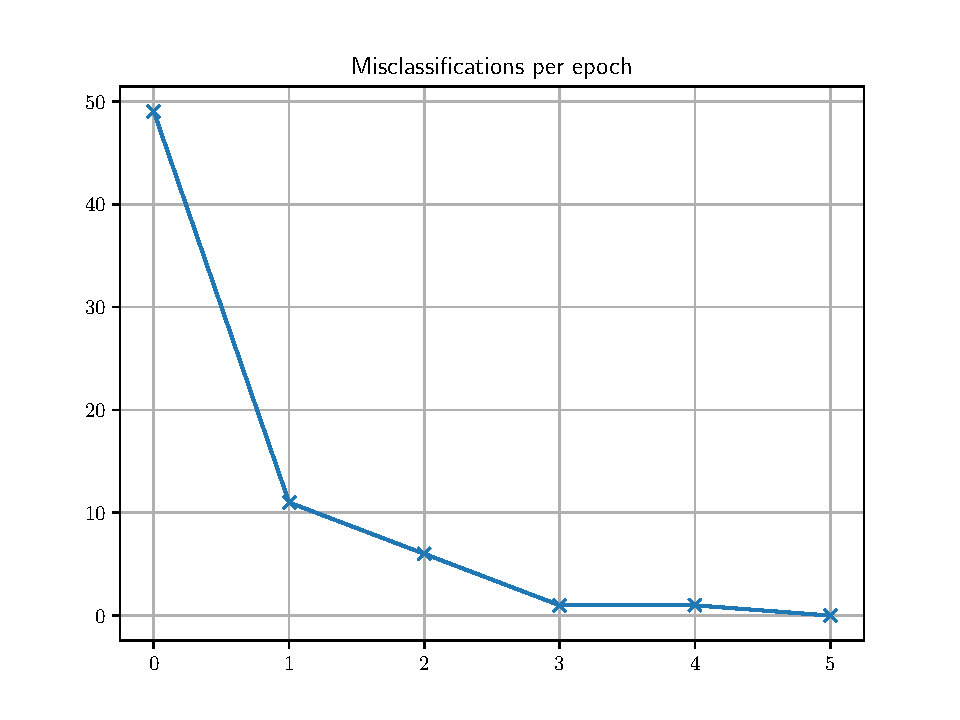
\includegraphics[width=.49\linewidth]{errors_50.pdf}
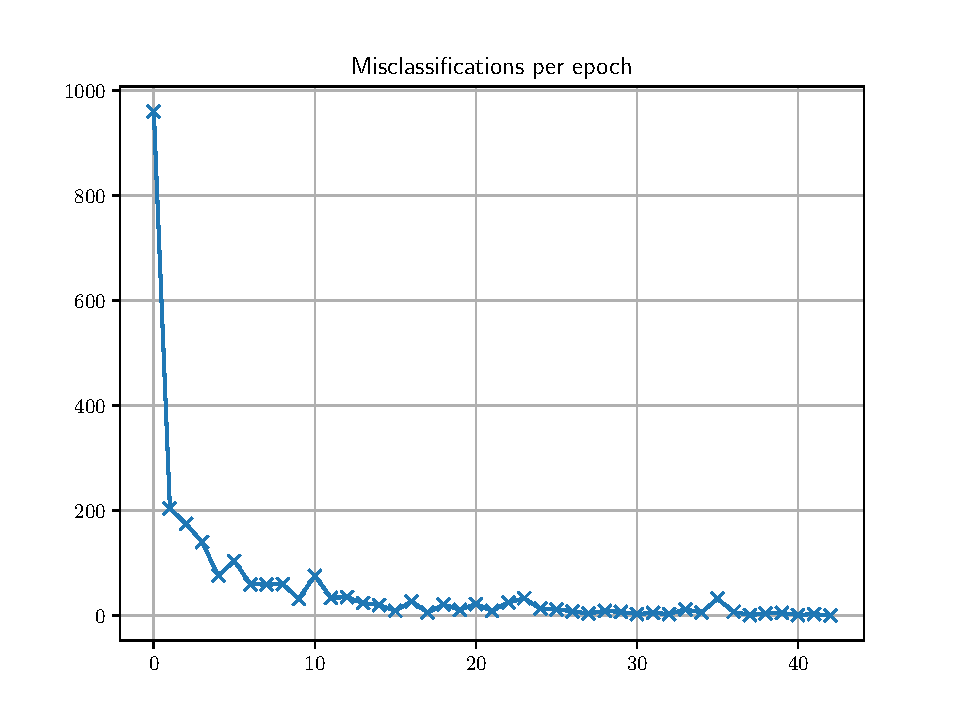
\includegraphics[width=.49\linewidth]{errors_1000.pdf}
\caption{Classification error rate per epoch ($n = 50, 1000$)}
\label{errors_50_1000}
\end{figure}

In the third run, the network is trained using the entire data set; in this case, the algorithm was not able to converge in a manageable number of epochs (epoch limit was set to 250). This is due to the size of the data set and to the probable impossibility to linearly separate the classes of interest: in fact, after the initial epochs, the error rate did not continue to show a decreasing tendency, but instead remained quite stable around 12\%-18\%. At the time the epoch limit was reached, the network still misclassified 8742 elements of the training set (14.570\%). 

In this case, we can see that the proportion of misclassified patterns for the training set matches more closely the results found for the test set (15.540\%, coming from 1554 misclassifications). This was somehow expected, since we are using all the data we have in the training set: given the greater dimension of the input set, in fact, this measure becomes statistically significant also for the training set (it was not in the previous cases, using a reduced number of samples).

\begin{figure}[h]
\centering
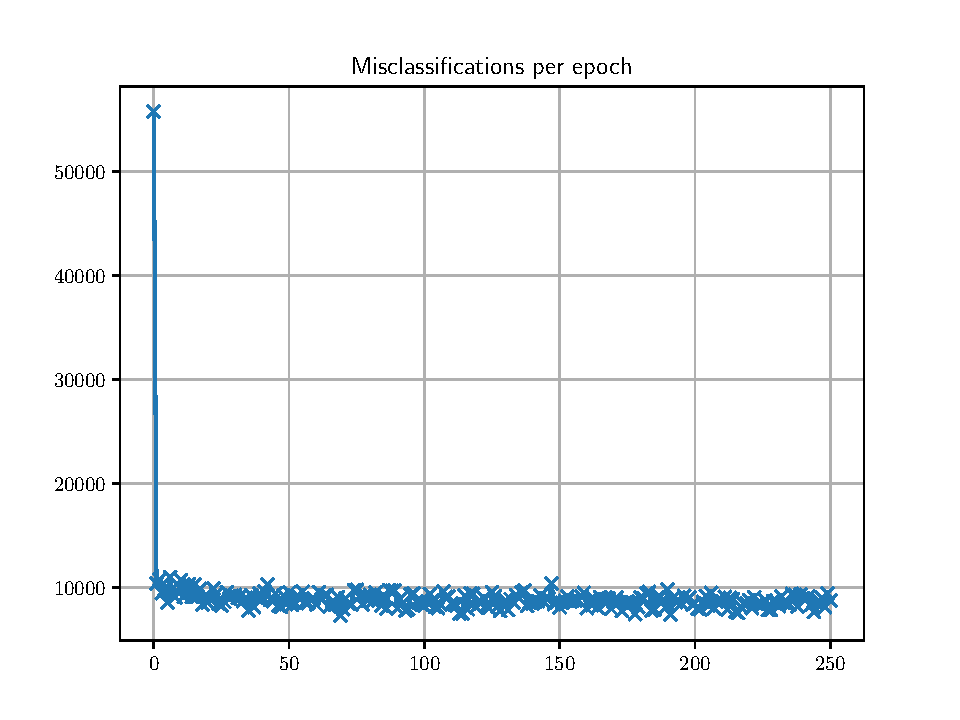
\includegraphics[width=.7\linewidth]{errors_60000.pdf}
\caption{Classification error rate per epoch ($n = 60000$)}
\label{errors_60000}
\end{figure}

\subsection{Results for variable $W_0$}

For the last part of the exercise, the training algorithm has been used to train a network after having fixed the values of $n = 60000$ (all training samples used), $\epsilon = 0.125$ (maximum error rate on the training set of 12.5\%) and $\eta = 5$. Three runs have been executed, all using different values for the matrix of the initial weights $W_0$. Results are shown in table \ref{results_varw}.

\begin{table}[h]
\centering
\begin{tabular}{|c|c|c|c|}
\hline
Run   & Epochs for convergence & Training set errors & Test set errors \\ \hline
1     & 114 & 7486 (12.477\%) & 1315 (13.150\%) \\ \hline
2     & 53  & 7387 (12.312\%) & 1293 (12.930\%) \\ \hline
3     & 182 & 7271 (12.118\%) & 1283 (12.830\%) \\ \hline
\end{tabular}
\caption{Results for the runs with variable $W_0$}
\label{results_varw}
\end{table}

As we can see, results for the three runs are quite close for all parameters except for the number of epochs required to make the algorithm converge. In fact, the Perceptron Training Algorithm is very dependent on the choice of initial weights; even in the cases in which it guarantees convergence (in case of linear separability of the classes), it may take more or less epochs to reach it. In the presented case, the second run was the one that required the least number of epochs to reach convergence (53).

As for the classification accuracy, we can see that, as in the previous case, results for training and test sets are quite close, which is expected since we are training the network with all the available training data. Of the three runs, the one that yielded the best results overall was the third, with a test set inaccuracy of 12.83\%.

\begin{figure}[h]
\centering
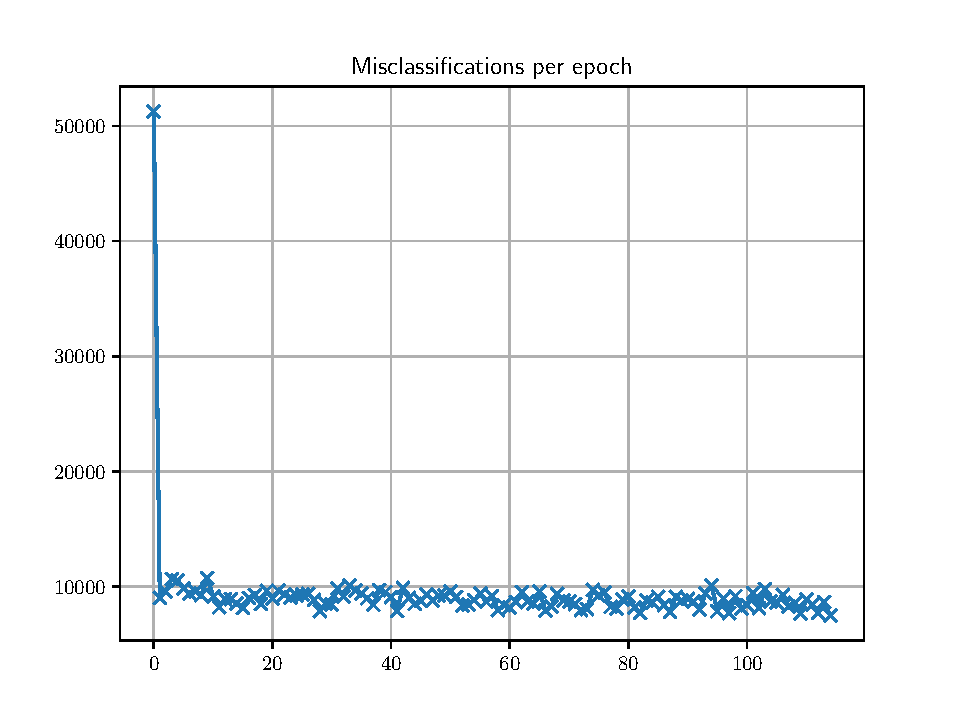
\includegraphics[width=.45\linewidth]{errors_60000_125_1.pdf}
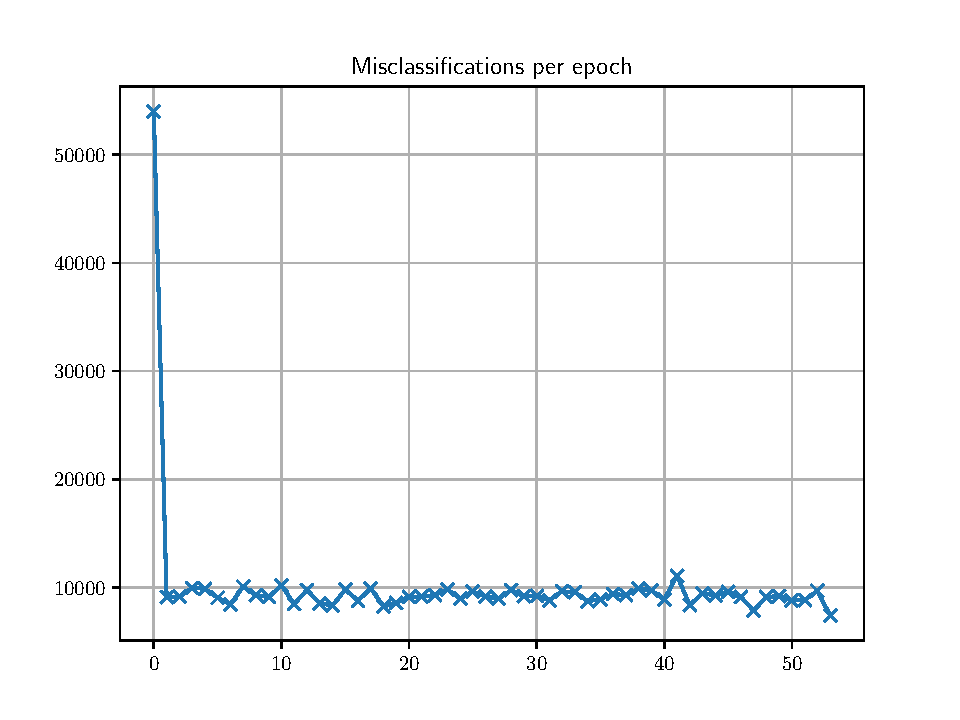
\includegraphics[width=.45\linewidth]{errors_60000_125_2.pdf}
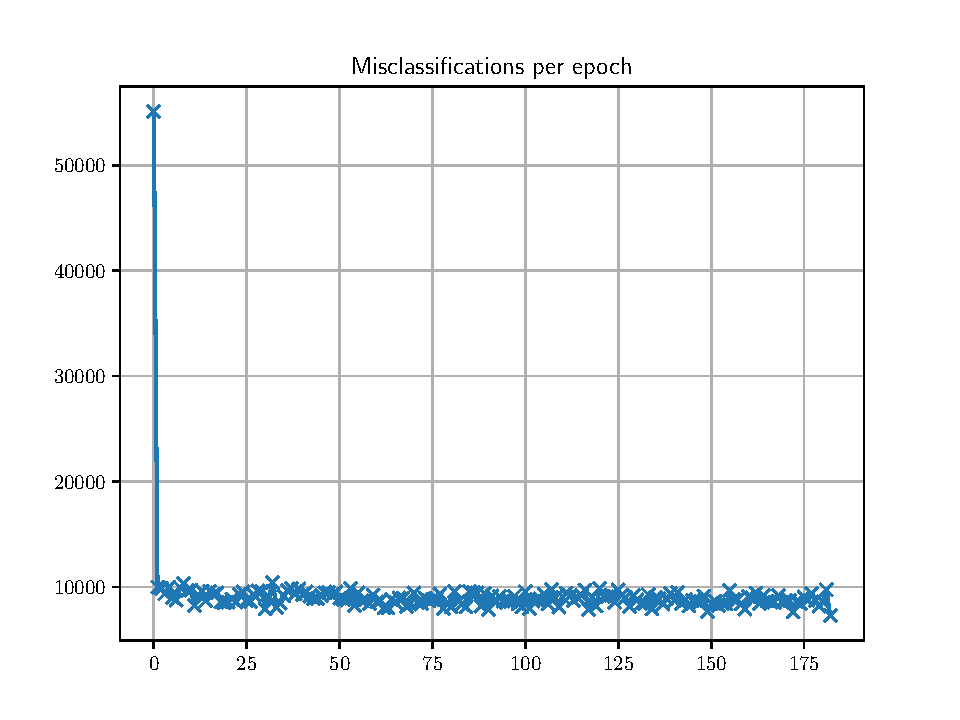
\includegraphics[width=.45\linewidth]{errors_60000_125_3.pdf}
\caption{Classification error rate per epoch (variable $W_0$)}
\label{errors_varw}
\end{figure}

\subsection{Complete Python code}

\lstinputlisting[basicstyle=\ttfamily\scriptsize]{hw2_ex2.py}

\end{document}